%% PREAMBLE %%

% document class
\documentclass[titlepage]{article}

% document layout packages 
\usepackage{geometry} % allows easier page formatting
\geometry{left=2.5cm,right=2.5cm,top=2.5cm,bottom=2.5cm}
\usepackage{tabularx} % table package
\usepackage{graphicx} % image package!


% symbol packages
\usepackage{amssymb} % lots of stuff ex: bbm !
\usepackage{siunitx}  % SI units

% math packages
\usepackage{amsmath} % amsmath package
\usepackage{nicefrac} % commands to make ugly fractions nicer. not always needed!
\usepackage{bm} % bold math package !

% formatting
\usepackage{indentfirst} % suppresses inbuilt "no-indent" after section
\usepackage{setspace} % Using \doublespacing in the preamble 
\usepackage{enumerate} % lists nd stuff 
\onehalfspacing % changes the text to 1.5-line spacing

% main font (inter light)
\usepackage[sfdefault,light]{inter} %% Option 'sfdefault' only if 'inter' is to be used
\usepackage[T1]{fontenc}

% math font package
\usepackage{amsfonts} % latex defaults fractions to main font, so must use \displaystyle before \frac expression

% other
\usepackage[english]{isodate} % date package
\usepackage[colorlinks=true, urlcolor=blue, linkcolor=red]{hyperref} % hyperlink package

\begin{document} % begin document!

%% TITLE PAGE %%
\title{\textbf{Module 3 Assignment}}
\author{Nathan Shea Ouedraogo}
\date{\printdateTeX{2024/04/18}}
\maketitle


%% QUESTION 1 %%
    \section{}
    \begin{center}
        \large
        \textbf{Dimensional Reduction of a Scalar Variable}
    \end{center}
    \normalsize

    \noindent A dimensional variable $u$ may be reduced to its non-dimensional form $\tilde{u}$ by re-centering it to the origin by a scalar $u_{r}$ and dividing it by a scalar factor $u_{s}$ :
    \begin{align}
        \tilde{u} &= \displaystyle\frac{u-u_{r}}{u_{s}}
    \end{align}

    \noindent If we assume that the variable is already centered at the origin, $u_{r}$ disappears:
    \begin{align}
        \tilde{u} &= \displaystyle\frac{u}{u_{s}}
    \end{align}

    \noindent Rearranging to put the equation in terms of the dimensional variable: 
    \begin{align}
        u_{s}\tilde{u} &= u\hspace*{5pt}\square
    \end{align}

    \begin{center}
        \large
        \textbf{Dimensional Reduction of a Vector Variable}
    \end{center}
    \normalsize

    \noindent Given a vector variable 
    $\vec{u}=\left<u_{1},u_{2},\cdots,u_{n-1}\right>,\hspace*{2pt}\vec{u_{n}}\hspace*{2pt}\in\hspace*{2pt}\mathbb{R}^n$ 
    with \emph{n} number of dimensional elements its non-dimensional form $\vec{\tilde{u}}$ is:

    \begin{align}
        \vec{\tilde{u}} &= \langle{\displaystyle\frac{u_{1}-u_{r_{1}}}{u_{s_{1}}}, \displaystyle\frac{u_{2}-u_{r_{2}}}{u_{s_{2}}}, \cdots, \displaystyle\frac{u_{n-1}-u_{r_{n-1}}}{u_{s_{n-1}}}}\rangle
    \end{align}

    \noindent If we assume the vector is centered at the origin, the equation becomes: 

    \begin{align}
        \vec{\tilde{u}}=\langle{\displaystyle\frac{u_{1}}{u_{s_{1}}}, \displaystyle\frac{u_{2}}{u_{s_{2}}}, \cdots, \displaystyle\frac{u_{n-1}}{u_{s_{n-1}}}}\rangle
    \end{align}

    \noindent If all  elements of $\vec{\tilde{u}}$ have the same dimension, we can scale some by a critical factor $U_{0}$:
    \begin{align}
        \vec{\tilde{u}} &= \langle{\displaystyle\frac{u_{1}}{U_{0}}, \displaystyle\frac{u_{2}}{U_{0}}, \cdots, \displaystyle\frac{u_{n-1}}{U_{0}}}\rangle \\
        \vec{\tilde{u}} &= \displaystyle\frac{1}{U_{0}}\langle{u_{1}, u_{2}, \cdots, u_{n-1}}\rangle
    \end{align}
    \noindent And finally we can rearrange the equation in terms of the dimensional vector: 

    \begin{align}
        U_{0}\vec{\tilde{u}} &= \langle{u_{1}, u_{2}, \cdots, u_{n-1}}\rangle \\
        U_{0}\vec{\tilde{u}} &= \vec{u}\hspace*{5pt}\square
    \end{align}

    \newpage

    \begin{center}
        \textbf{\emph{i) Navier-Stokes Equations for Incompressible Liquids}}
    \end{center}
    \begin{align}
        \rho\left(\displaystyle\frac{\partial\vec{v}}{\partial{t}}\right)+\left(\vec{v}\cdot\vec{\nabla}\right)\vec{v} &= -\vec{\nabla}p+\eta\nabla^2\vec{v}+\rho\vec{F}
    \end{align}

    \begin{center}
        \textbf{\emph{ii) Dimensional Reduction of Time and Pressure}}
    \end{center}

    Applying Equation (1):
    \begin{align}
        \tilde{t}  &=  \displaystyle\frac{t-t_{r}}{t_{s}} \\
        \tilde{p}  &=  \displaystyle\frac{p-p_{r}}{p_{s}}
    \end{align}

    Applying Equation (2):
    \begin{align}
        \tilde{t}  &=  \displaystyle\frac{t}{t_{s}} \\
        \tilde{p}  &=  \displaystyle\frac{p}{p_{s}}
    \end{align}

    Applying Equation (3):
    \begin{align}
        t_{s}\tilde{t}  &= t\\
        p_{s}\tilde{p} &= p\hspace*{5pt}\square 
    \end{align} 
    \begin{center}
        \textbf{\emph{iii) Dimensional Reduction of Velocity}}
    \end{center}

    \noindent The dimensional velocity vector is:

    \begin{align}
        \vec{v} &= \begin{bmatrix}
            v_{x} \\
            v_{y} \\
            v_{z} 
        \end{bmatrix}
    \end{align}

    \noindent Applying equation (4) gives the dimensionless velocity vector:
    \begin{align}
        \vec{\tilde{v}} &= \begin{bmatrix}
            \displaystyle\frac{v_{x}-v_{r_{x}}}{v_{s_{x}}} \\[10pt]
            \displaystyle\frac{v_{y}-v_{r_{y}}}{v_{s_{y}}} \\[10pt]
            \displaystyle\frac{v_{y}-v_{r_{y}}}{v_{s_{y}}} 
        \end{bmatrix}
    \end{align}

    \newpage
    \noindent Given a critical velocity $V_{0}$ and using equations (5) \& (9): 
    \begin{align}
        \vec{\tilde{v}} &= \displaystyle\frac{1}{V_{0}}\begin{bmatrix}
            v_{x} \\
            v_{y} \\
            v_{z}     
        \end{bmatrix} \\
        {V_{0}}\vec{\tilde{v}} &= \vec{v}\hspace*{5pt}\square
    \end{align}

    \begin{center}
        \textbf{\emph{iv) Dimensional Reduction of the Position Vector}}
    \end{center}
    The position vector is: 
    \begin{align}
        \vec{f} &= \begin{bmatrix}
            x \\
            y \\
            z 
        \end{bmatrix}
    \end{align}
    \noindent Which by equations (4)-(7) and a critical length of $L_{0}$ gives the relationship: 
    \begin{align}
        \vec{f}=L_{0}\vec{\tilde{f}}\hspace*{5pt}
        =L_{0}\begin{bmatrix}
            \tilde{x} \\
            \tilde{y} \\
            \tilde{z}
        \end{bmatrix}
        =\begin{bmatrix}
            L_{0}\tilde{x}\\
            L_{0}\tilde{y} \\
            L_{0}\tilde{z}
        \end{bmatrix}
        = \begin{bmatrix}
            x \\
            y \\
            z 
        \end{bmatrix}
        =\vec{f} \hspace*{5pt}\square
    \end{align}

    \begin{center}
        \textbf{\emph{v) Dimensional Reduction of the Pressure Gradient}}
    \end{center}

    \noindent The dimensional pressure gradient is:
    \begin{align}
        -\vec{\nabla}p &= -\begin{bmatrix}
            \displaystyle\frac{\partial{f\left(x,y,z\right)}}{\partial{x}}p_{x} \\[0.4cm]
            \displaystyle\frac{\partial{f\left(x,y,z\right)}}{\partial{y}}p_{y} \\[0.4cm]
            \displaystyle\frac{\partial{f\left(x,y,z\right)}}{\partial{z}}p_{z}
        \end{bmatrix}
    \end{align}

    \noindent And its dimensionless form:  
    \begin{align}
        -\vec{\tilde{\nabla}}\tilde{p} &= -\begin{bmatrix}
            \displaystyle\frac{\partial{\tilde{f}\left(\tilde{x},\tilde{y},\tilde{z}\right)}}{\partial{\tilde{x}}}\tilde{p}_{x} \\[0.4cm]
            \displaystyle\frac{\partial{\tilde{f}\left(\tilde{x},\tilde{y},\tilde{z}\right)}}{\partial{\tilde{y}}}\tilde{p}_{y} \\[0.4cm]
            \displaystyle\frac{\partial{\tilde{f}\left(\tilde{x},\tilde{y},\tilde{z}\right)}}{\partial{\tilde{z}}}\tilde{p}_{z} 
        \end{bmatrix}
    \end{align}

    \noindent Substituting dimensionless quantities from equations (16), (22) into equation (23) gives: 
    \begin{align}
        -\vec{\nabla}p &= -\begin{bmatrix}
            \displaystyle\frac{\partial{\tilde{f}\left(\tilde{x},\tilde{y},\tilde{z}\right)}}{\partial{L_{0}\tilde{x}}}p_{s}\tilde{p}_{x} \\[0.4cm]
            \displaystyle\frac{\partial{\tilde{f}\left(\tilde{x},\tilde{y},\tilde{z}\right)}}{\partial{L_{0}\tilde{y}}}p_{s}\tilde{p}_{y} \\[0.4cm]
            \displaystyle\frac{\partial{\tilde{f}\left(\tilde{x},\tilde{y},\tilde{z}\right)}}{\partial{L_{0}\tilde{z}}}p_{s}\tilde{p}_{z} 
        \end{bmatrix}
    \end{align}



    \noindent Since the critical length is a constant, it can be pulled out: 
    \begin{align}
        -\vec{\nabla}p &= -\displaystyle\frac{1}{L_{0}}\begin{bmatrix}
            \displaystyle\frac{\partial{\tilde{f}\left(\tilde{x},\tilde{y},\tilde{z}\right)}}{\partial{\tilde{x}}}p_{s_{x}}\tilde{p}_{x} \\[0.4cm]
            \displaystyle\frac{\partial{\tilde{f}\left(\tilde{x},\tilde{y},\tilde{z}\right)}}{\partial{\tilde{y}}}p_{s_{y}}\tilde{p}_{y} \\[0.4cm]
            \displaystyle\frac{\partial{\tilde{f}\left(\tilde{x},\tilde{y},\tilde{z}\right)}}{\partial{\tilde{z}}}p_{s_{z}}\tilde{p}_{z} 
        \end{bmatrix}
    \end{align}

    \noindent And by equation (24) gives:
    \begin{align}
        -\vec{\nabla}p &= -\displaystyle\frac{1}{L_{0}}\vec{\tilde{\nabla}}p_{s}\tilde{p}\hspace*{5pt}\square
    \end{align}

    \begin{center}
        \textbf{\emph{vi) Dimensional Reduction of the Dynamic Viscosity Field}}
    \end{center}

    \noindent The dynamic viscosity field is given by: 
    \begin{align}
        \eta\nabla^2\vec{v} &=\eta\begin{bmatrix}
            \displaystyle\frac{\partial^{\hspace*{1pt}2}{f\left(x,y,z\right)}}{\partial{x^{2}}}v_{x} \\[0.4cm]
            \displaystyle\frac{\partial^{\hspace*{1pt}2}{f\left(x,y,z\right)}}{\partial{y^{2}}}v_{y}  \\[0.4cm]
            \displaystyle\frac{\partial^{\hspace*{1pt}2}{f\left(x,y,z\right)}}{\partial{z^{2}}}v_{z}
        \end{bmatrix}
    \end{align}

    \noindent And when dimensionally reduced: 

    \begin{align}
        {\eta}\tilde{\nabla}^2\vec{\tilde{v}} &= {\eta}\begin{bmatrix}
            \displaystyle\frac{\partial^{\hspace*{1pt}2}{\tilde{f}\left(\tilde{x},\tilde{y},\tilde{z}\right)}}{\partial{\tilde{x}^{2}}}\tilde{v_{x}} \\[0.4cm]
            \displaystyle\frac{\partial^{\hspace*{1pt}2}{\tilde{f}\left(\tilde{x},\tilde{y},\tilde{z}\right)}}{\partial{\tilde{y}^{2}}}\tilde{v_{y}}  \\[0.4cm]
            \displaystyle\frac{\partial^{\hspace*{1pt}2}{\tilde{f}\left(\tilde{x},\tilde{y},\tilde{z}\right)}}{\partial{\tilde{z}^{2}}} \tilde{v_{z}}
        \end{bmatrix}
    \end{align}

    \newpage
    \noindent Substituting equation (22) into equation (28) with a critical velocity $V_{0}$ gives: 

    \begin{align}
        \eta\nabla^2\vec{v} &={\eta}\begin{bmatrix}
            \displaystyle\frac{\partial^{\hspace*{1pt}2}{\tilde{f}\left(\tilde{x},\tilde{y},\tilde{z}\right)}}{\partial{\left(L_{0}\tilde{x}\right)^{2}}}{V_{0}}\vec{\tilde{v_{x}}} \\[0.45cm]
            \displaystyle\frac{\partial^{\hspace*{1pt}2}{\tilde{f}\left(\tilde{x},\tilde{y},\tilde{z}\right)}}{\partial{\left(L_{0}\tilde{y}\right)^{2}}}{V_{0}}\vec{\tilde{v_{y}}}  \\[0.45cm]
            \displaystyle\frac{\partial^{\hspace*{1pt}2}{\tilde{f}\left(\tilde{x},\tilde{y},\tilde{z}\right)}}{\partial{\left(L_{0}\tilde{z}\right)^{2}}}{V_{0}}\vec{\tilde{v_{z}}}
        \end{bmatrix} 
    \end{align}

    \noindent Pulling out the critical length and velocity:
    \begin{align}
        \eta\nabla^2\vec{v} &= \displaystyle\frac{\eta{V_{0}}}{L_{0}^2}\begin{bmatrix}
            \displaystyle\frac{\partial^{\hspace*{1pt}2}{\tilde{f}\left(\tilde{x},\tilde{y},\tilde{z}\right)}}{\partial{\tilde{x}^{2}}}\vec{\tilde{v_{x}}} \\[0.45cm]
            \displaystyle\frac{\partial^{\hspace*{1pt}2}{\tilde{f}\left(\tilde{x},\tilde{y},\tilde{z}\right)}}{\partial{\tilde{y}^{2}}}\vec{\tilde{v_{y}}}  \\[0.45cm]
            \displaystyle\frac{\partial^{\hspace*{1pt}2}{\tilde{f}\left(\tilde{x},\tilde{y},\tilde{z}\right)}}{\partial{\tilde{z}^{2}}}\vec{\tilde{v_{z}}}
        \end{bmatrix}
    \end{align}

    \noindent And finally, substituting equation (29): 
    \begin{align}
        \eta\nabla^2\vec{v} &= \displaystyle\frac{\eta{V_{0}}}{L_{0}^2}\tilde{\nabla}^2\vec{\tilde{v}}\hspace*{5pt}\square
    \end{align}  \\  \\

    \begin{center}
        \textbf{\emph{vii) The Reynolds Number (Re)}}
    \end{center}

    \noindent The Reynolds number is a scalar value which modulates the dimensionless velocity gradient: 

    \begin{align}
        Re &= \rho\left(\displaystyle\frac{L_{0}V_{0}}{\eta}\right)
    \end{align}

    \noindent In the following section we will see how this number is applied.

    \newpage
    \begin{center}
        \textbf{\emph{viii) Non-Dimensional Navier-Stokes Equations}}
    \end{center}

    \noindent Substituting equations (15), (16), (20), (27), and (32) into equation (10) gives: 

    \begin{align}
        \rho\left(
            \displaystyle\frac{\partial{V_{0}\vec{\tilde{v}}}}{\partial{t_{s}\tilde{t}}}+\vec{\tilde{v}}\left(\vec{\tilde{\nabla}}\cdot\vec{\tilde{v}}\right)
        \right) 
        &= -\displaystyle\frac{1}{L_{0}}\vec{\tilde{\nabla}}p_{s}\tilde{p} + \displaystyle\frac{\eta{V_{0}}}{L_{0}^2}\tilde{\nabla}^2\vec{\tilde{v}} + \rho\vec{F} \\
        \rho\left(
            \displaystyle\frac{V_{0}}{t_{s}} 
            \right)\left(\displaystyle\frac{\partial{\vec{\tilde{v}}}}{\partial{\tilde{t}}}\right) + \rho\left(\vec{\tilde{v}}\left(\vec{\tilde{\nabla}}\cdot\vec{\tilde{v}}\right)
        \right)
        &= -\displaystyle\frac{1}{L_{0}}\vec{\tilde{\nabla}}p_{s}\tilde{p} + \displaystyle\frac{{\eta}{V_{0}}}{L_{0}^2}\tilde{\nabla}^2\vec{\tilde{v}} + \rho\vec{F}
    \end{align}

    \noindent Dividing by the highest order derivative term and assuming negligible contribution from body forces: 
    \begin{align}
        \left(
            \displaystyle\frac{L_{0}^2}{\eta{V_{0}}}
        \right)
        \rho\left(
            \displaystyle\frac{V_{0}}{t_{s}} 
            \right)\left(\displaystyle\frac{\partial{\vec{\tilde{v}}}}{\partial{\tilde{t}}}\right) + \vec{\tilde{v}}\left(\vec{\tilde{\nabla}}\cdot\vec{\tilde{v}}\right)
        &= \left(\displaystyle\frac{L_{0}^2}{\eta{V_{0}}}\right)\left(-\displaystyle\frac{1}{L_{0}}\vec{\tilde{\nabla}}p_{s}\tilde{p}\right) + \left(
            \displaystyle\frac{L_{0}^2}{\eta{V_{0}}}
        \right) \displaystyle\frac{{\eta}{V_{0}}}{L_{0}^2}\tilde{\nabla}^2\vec{\tilde{v}}  \\
        \rho\left(\displaystyle\frac{L_{0}^2}{\eta}\right)\left(\displaystyle\frac{\partial{\vec{\tilde{v}}}}{\partial{\tilde{t}}}\right) + \rho\left(\displaystyle\frac{L_{0}V_{0}}{\eta}\right)\left(\vec{\tilde{v}}\left(\vec{\tilde{\nabla}}\cdot\vec{\tilde{v}}\right)\right) &= -\displaystyle\frac{L_{0}}{\eta{V_{0}}}\vec{\tilde{\nabla}}p_{s}\tilde{p} + \tilde{\nabla}^2\vec{\tilde{v}}
    \end{align}


    \noindent And finally applying equation (33) to equation (37): 
    \begin{align}
        \rho\left(\displaystyle\frac{L_{0}^2}{\eta}\right)\left(\displaystyle\frac{\partial{\vec{\tilde{v}}}}{\partial{\tilde{t}}}\right) + Re\left[\vec{\tilde{v}}\left(\vec{\tilde{\nabla}}\cdot\vec{\tilde{v}}\right)\right] &= -\displaystyle\frac{L_{0}}{\eta{V_{0}}}\vec{\tilde{\nabla}}p_{s}\tilde{p} + \tilde{\nabla}^2\vec{\tilde{v}} \hspace*{5pt}\blacksquare
    \end{align}

%% QUESTION 2 %%
\newpage
\section{}
    \noindent Per equation (33) $Re$ is defined as: 
    \begin{align*}
        Re &= \rho\left(\displaystyle\frac{L_{0}V_{0}}{\eta}\right)
    \end{align*}
    \noindent  Where $L_{0}$ and $V_{0}$ are critical length (hydrodynamic diameter) and critical velocity respectively, and $\rho$ and $\eta$ are the density and dynamic viscosity of the fluid respectively If pressure and temperature are assumed to be constant and body forces are assumed to be negligible, $\rho$ and $\eta$ can be assumed to be constants. $Re$ is therefore dependent on two forces; viscosity forces dependent on $\rho$ and $\eta$ and inertial forces dependent on $L_{0}$ and $V_{0}$. We can construct two simplified mental models of the physical effect of $Re$ using our intuition and own experience. We know that viscous fluids like honey have a greater tendency to `stick' and less tendency to `flow'. When honey does flow it is slow and smooth with little bubbles or turbulence. However, upon heating honey it becomes much easier to pour which can be modeled as increasing the fluid's velocity. The flow of hot honey is noticeably more chaotic with bubbles and turbulence. Another way to increase this observed chaos would be to increase the diameter of the flowing liquid; honey flowing from the tip of a squeeze bottle is much more smooth than honey flowing from an upturned jar. \\ \\ 
    \noindent In the first model where fluid flow is `smooth', the system is dominated by viscosity forces ($Re < 1$) and the fluid flow is said to be laminar:
    \begin{align}
        \displaystyle\frac{\rho}{\eta} > L_{0}V_{0}
    \end{align}
    \noindent The second model with `chaotic' flow is dominated by inertial forces ($Re$>{}>1) and the flow is said to be turbulent: 
    \begin{align}
        \displaystyle\frac{\rho}{\eta} << L_{0}V_{0}
    \end{align}
    \noindent Intermediate values are neither fully turbulent nor fully laminar and have contributions by both forces. 

%% QUESTION 3 %%
\newpage
\section{}
    \begin{center}
        \large
        \textbf{Hagen-Poiseuille Flow between Parallel Plates}
    \end{center}
    \normalsize
    \noindent Given a cross section perpendicular to the flow of the fluid, $\partial\hspace*{2pt}\mathcal{C}$, the flow is said to be under Hagen-Poiseuille conditions if: 
    \small
    \begin{center}
        \emph{\begin{enumerate}
            \item The system is translationally invariant in the direction of the flow
            \item Pressure is applied in one direction
            \item No body forces act upon the system
            \item For a given cross-section of a pipe, $\mathcal{C}$, the velocity at any point along the wall, $\partial\hspace*{2pt}\mathcal{C}$, is zero (no-slip condition)
            \item Pressure boundary conditions hold: $p(t_{i})=p_{0}+\Delta{p}$, $p(t_{f})=p_{0}$
        \end{enumerate}}
    \end{center}
    \vspace*{10pt}
    \normalsize
    \begin{center}
        \textbf{\emph{i) Navier-Stokes Equations for Incompressible Liquids in Cartesian Coordinates}}
    \end{center}

    \noindent The convective term of the Navier Stokes equation (eq. 10) is: 

    \begin{align*}
        \left(\vec{v}\cdot\vec{\nabla}\right)\vec{v}
    \end{align*}

    \noindent If we choose the z-axis as our translationally invariant axis, we can ignore the x and y equations of the Navier-Stokes equations since they will not contribute to the flow of the system. Equation (10) reduces to: 

    \begin{align}
        \left(\vec{v}_{z}\cdot\vec{\nabla}_{z}\right)\vec{v}_{z}&=v_{x}\left(\displaystyle\frac{\partial}{\partial{x}}v_{z}\vec{i}\right)+v_{y}\left(\displaystyle\frac{\partial}{\partial{y}}v_{z}\vec{j}\right)+v_{z}\left(\displaystyle\frac{\partial}{\partial{z}}v_{z}\vec{k}\right)
    \end{align}

    \noindent Since the velocity vector is dependent only on pressure, it will only point along the z-axis and be zero everywhere else. Thus equation (41) reduces to:

    \begin{align}
        \left(\vec{v}_{z}\cdot\vec{\nabla}_{z}\right)\vec{v}_{z}=\left(0\right)\left(\displaystyle\frac{\partial}{\partial{x}}v_{z}\vec{i}\right)+\left(0\right)\left(\displaystyle\frac{\partial}{\partial{y}}v_{z}\vec{j}\right)+v_{z}\left(\displaystyle\frac{\partial}{\partial{z}}v_{z}\vec{k}\right) 
        =v_{z}\left(\displaystyle\frac{\partial}{\partial{z}}v_{z}\vec{k}\right) 
    \end{align}

    \noindent And finally, since the z-axis is translationally invariant, the change in velocity is zero:
    \begin{align}
        \left(\vec{v}_{z}\cdot\vec{\nabla}_{z}\right)\vec{v}_{z}=\left(0\right)\left(\displaystyle\frac{\partial}{\partial{z}}v_{z}\vec{k}\right)=0\hspace*{5pt}\blacksquare
    \end{align}

    \noindent By equation (43), a system under Hagen-Poiseuille flow has no convection and is therefore laminar. 

    \newpage
    \noindent  Since convection is zero under Hagen-Poiseuille flow, pressure is the only force which will be acting on our system. Additionally, pressure will only be acting along the z-axis. Applying equation (43) to equation (10): 

    \begingroup
        \addtolength\jot{5pt}
        \begin{align}
            0&=-\vec{\nabla}p+\eta\nabla^2\vec{v_{z}}\\   
            \displaystyle\frac{\partial{p}}{\partial{x}}+\displaystyle\frac{\partial{p}}{\partial{y}}+\frac{\partial{p}}{\partial{z}}&=\eta\left(\displaystyle\frac{\partial^2{v_{z}}}{\partial{x}^2}+\displaystyle\frac{\partial^2{v_{z}}}{\partial{y}^2}+\displaystyle\frac{\partial^2{v_{z}}}{\partial{z}^2}\right) \\ 
            \displaystyle\frac{\partial{p}}{\partial{z}}&=\eta\left(\frac{\partial^2{v_{z}}}{\partial{x}^2}+\displaystyle\frac{\partial^2{v_{z}}}{\partial{y}^2}+\frac{\partial^2{v}}{\partial{z}^2}\right) \\
        \displaystyle\frac{\partial{p}}{\partial{z}}&=\eta\left(\displaystyle\frac{\partial^2{v_{z}}}{\partial{y}^2}\right)\hspace*{5pt}\blacksquare 
    \end{align} \\

    \begin{center}
        \textbf{\emph{ii) Derivation of Velocity}}
    \end{center}

    \noindent \noindent Given Hagen-Poiseuille flow, the velocity on $\partial\hspace*{2pt}\mathcal{C}$ is zero. Moving away from $\partial\hspace*{2pt}\mathcal{C}$ towards the center of the cross section $\mathcal{C}$ will increase the velocity with a maxima at the center of $\mathcal{C}$. We will define this center point as $y_{0}=0$ . Physically, the decrease in velocity as we approach the wall of the pipe is due to sheer stress along the pipe walls increasing drag and therefore decreasing velocity. Since velocity is symmetrical about $y_{0}$ the change in velocity with respect to position will be zero, $\displaystyle\frac{\partial{v_{z}}}{\partial{y}} = 0$. Applying to equation (47) gives a simple second-order ordinary differential equation:

    \begingroup
        \addtolength\jot{6pt}
        \begin{align}
            \int{\eta\displaystyle\frac{\partial^2{v_{z}}}{\partial{y}^2}dy}&=\int{\displaystyle\frac{\partial{p}}{\partial{z}}dy}\\
            \eta\displaystyle\frac{\partial{v_{z}}}{\partial{y}} + C_{0}&=\displaystyle\frac{\partial{p}}{\partial{z}}y \\
            C_{0} &=  \left(\displaystyle\frac{\partial{p}}{\partial{z}}\right)\left(\displaystyle\frac{y_{0}}{\eta}\right) - \displaystyle\frac{\partial{v_{z_{0}}}}{\partial{y}} \\
            C_{0} &=  \left(\displaystyle\frac{\partial{p}}{\partial{z}}\right)\left(\displaystyle\frac{0}{\eta}\right) - 0 \\
            C_{0} &=  0 \\
            \therefore \displaystyle\frac{\partial{p}}{\partial{z}}y&=\eta\displaystyle\frac{\partial{v_{z}}}{\partial{y}} \hspace*{5pt}\square 
        \end{align}
        
        \newpage
        \noindent The no-slip boundary condition states that the velocity on $\partial\hspace*{2pt}\mathcal{C}$ is zero. Let us define the vertical position at the boundary as $y_{1}$ and the velocity at the boundary as $v_{z_{1}}=0$. Applying to equation (53) leaves a first-order ordinary differential equation:
        \begin{align}
            \int{\eta\displaystyle\frac{\partial{v_{z}}}{\partial{y}}dy}&=\int{\displaystyle\frac{\partial{p}}{\partial{z}}ydy} \\
            v_{z}&= \left(\displaystyle\frac{y^2}{2\eta}\right)\left(\displaystyle\frac{\partial{p}}{\partial{z}}\right) + C_{1} \\
            C_{1} &= v_{z_{1}}-\left(\displaystyle\frac{y_{1}^2}{2\eta}\right)\left(\displaystyle\frac{\partial{p}}{\partial{z}}\right) \\
            C_{1}  &=-\left(\displaystyle\frac{y_{1}^2}{2\eta}\right)\left(\displaystyle\frac{\partial{p}}{\partial{z}}\right)\\
            v_{z}  &= \left(\displaystyle\frac{y^2}{2\eta}\right)\left(\displaystyle\frac{\partial{p}}{\partial{z}}\right) -\left(\displaystyle\frac{y_{1}^2}{2\eta}\right)\left(\displaystyle\frac{\partial{p}}{\partial{z}}\right) \\
            \therefore  v_{z} &= -\left(\displaystyle\frac{y_{1}^2}{2\eta}\right)\left(\displaystyle\frac{\partial{p}}{\partial{z}}\right)\left(1-\displaystyle\frac{y^2}{y_{1}^2}\right)\hspace*{5pt}\blacksquare
        \end{align}
    \endgroup \\

    \begin{center}
        \textbf{\emph{iii) Compliance with No-Slip Conditions}}
    \end{center}
    If the velocity is non-zero on the boundary of $\mathcal{C}$ , then the velocity will not be symmetrical. Physically this is due to the fluid experiencing shear stress and drag across the wall which causes non-zero velocity at the wall (`slip') and non-symmetrical velocity. No-slip conditions hold that the velocity at the wall is zero. This is trivial to prove as $y^2=y_{1}^2$ on $\partial\hspace*{2pt}\mathcal{C}$. Substituting into equation  (59) gives: 

    \begin{align}
        v_{z} &= -\left(\displaystyle\frac{y_{1}^2}{2\eta}\right)\left(\displaystyle\frac{\partial{p}}{\partial{z}}\right)\left(1-\displaystyle\frac{y_{1}^2}{y_{1}^2}\right) \\
        v_{z} &= -\left(\displaystyle\frac{y_{1}^2}{2\eta}\right)\left(\displaystyle\frac{\partial{p}}{\partial{z}}\right)\left(1-1\right) \\
        v_{z} &= -\left(\displaystyle\frac{y_{1}^2}{2\eta}\right)\left(\displaystyle\frac{\partial{p}}{\partial{z}}\right)\left(0\right) \\
        \therefore v_{z} &= 0 \hspace*{5pt} \blacksquare
    \end{align}

    \newpage
    \begin{center}
        \large
        \textbf{Hagen-Poiseuille Flow in a Circular Channel} \\
    \end{center}

    \normalsize
    \begin{center}
        \textbf{\emph{i) Navier-Stokes Equation for Incompressible Liquids in Cylindrical Coordinates}}
    \end{center}

    \noindent Mapping the cartesian z-component from equation (10) to cylindrical coordinates gives: 

    \begin{align}
        \rho\left(\displaystyle\frac{\partial{v_{z}}}{\partial{t}}+v_{r}\displaystyle\frac{\partial{v_{z}}}{\partial{r}}+\left(\displaystyle\frac{v_{\theta}}{r}\right)\left(\displaystyle\frac{\partial{v_{z}}}{\partial{\theta}}\right)+v_{z}\displaystyle\frac{\partial{v_{z}}}{\partial{z}}\right)&=-\displaystyle\frac{\partial{p}}{\partial{z}}+\eta\nabla^2v_{z}+\rho{g_{z}}
    \end{align}

    \noindent Given Hagen-Poiseuille flow this reduces to:
    \begin{align}    
        \displaystyle\frac{\partial{p}}{\partial{z}}&=\eta\nabla^2v_{z} \\ 
        \displaystyle\frac{\partial{p}}{\partial{z}}&=\eta\left[\displaystyle\frac{1}{r}\left(\displaystyle\frac{\partial}{\partial{r}}\right)\left(r\displaystyle\frac{\partial{v_{z}}}{\partial{r}}\right)+\displaystyle\frac{1}{r^2}\left(\displaystyle\frac{\partial^2{v_{z}}}{\partial{\theta^2}}\right)+\displaystyle\frac{\partial^2{v_{z}}}{\partial{z^2}}\right] \\
        \displaystyle\frac{\partial{p}}{\partial{z}}&=\displaystyle\frac{\eta}{r}\left[\left(\displaystyle\frac{\partial}{\partial{r}}\right)\left(r\displaystyle\frac{\partial{v_{z}}}{\partial{r}}\right)\right] \\
        \left(\displaystyle\frac{r}{\eta}\right)\left(\displaystyle\frac{\partial{p}}{\partial{z}}\right)dr&=\partial\left(r\displaystyle\frac{\partial{v_{z}}}{\partial{r}}\right)\hspace*{5pt}\square
        \end{align}
    \\
    \begin{center}
        \textbf{\emph{ii) Derivation of Velocity}}
    \end{center}
    \noindent Equations (47) \& (68) are analogous, so the method used to derive equation (53) may be used here as well. As with equation (47) let the boundary conditions be $r_{0}=0$, $v_{z_{0}}=0$:
    \begingroup
        \addtolength\jot{6pt}
        \begin{align}
            \int{\left(\displaystyle\frac{r}{\eta}\right)\left(\displaystyle\frac{\partial{p}}{\partial{z}}\right)dr}&=\int{\partial\left(r\displaystyle\frac{\partial{v_{z}}}{\partial{r}}\right)} \\
            \left(\displaystyle\frac{r^2}{2\eta}\right)\left(\frac{\partial{p}}{\partial{z}}\right)&=r\left(\displaystyle\frac{\partial{v_{z}}}{\partial{r}}\right)+C_{0}\\
            \because C_{0}&=\left(\displaystyle\frac{r_{0}^2}{2\eta}\right)\left(\frac{\partial{p}}{\partial{z}}\right)-r_{0}\left(\displaystyle\frac{\partial{v_{z}}}{\partial{r_{0}}}\right)=0\\
            \therefore\left(\displaystyle\frac{r^2}{2\eta}\right)\left(\frac{\partial{p}}{\partial{z}}\right)&=r\left(\displaystyle\frac{\partial{v_{z}}}{\partial{r}}\right)\hspace*{5pt}\square
        \end{align}
    \endgroup

    \newpage

    \noindent Equations (72) \& (53) are analogous, so the same method applies:
    \begingroup
        \addtolength\jot{6pt}
        \begin{align}
            \int{\left(\displaystyle\frac{r^2}{2\eta}\right)\left(\frac{\partial{p}}{\partial{z}}\right)dr}&=\int{r\left(\displaystyle\frac{\partial{v_{z}}}{\partial{r}}\right)}\\
            v_{z} &= \left(\displaystyle\frac{r^2}{4\eta}\right)\left(\displaystyle\frac{\partial{p}}{\partial{z}}\right)+C_{1}\\
            C_{1} &= v_{z_{1}} - \left(\displaystyle\frac{r_{1}^2}{4\eta}\right)\left(\displaystyle\frac{\partial{p}}{\partial{z}}\right) \\
            C_{1} &= - \left(\displaystyle\frac{r_{1}^2}{4\eta}\right)\left(\displaystyle\frac{\partial{p}}{\partial{z}}\right) \\
            \therefore v_{z}\left(r,\theta\right) &= -\left(\displaystyle\frac{1}{4\eta}\right)\left(\displaystyle\frac{\partial{p}}{\partial{z}}\right)\left(r_{1}^2-r^2\right)\hspace*{5pt}\blacksquare
        \end{align}
    \endgroup \\

    \begin{center}
        \textbf{\emph{iii) Compliance with No-Slip Conditions}}
    \end{center}

    \noindent By setting the radius $\left(r^2\right)$ to the boundary, from equation we get (77):
    \begin{align}
        v_{z}\left(r,\theta\right) &= -\left(\displaystyle\frac{1}{4\eta}\right)\left(\displaystyle\frac{\partial{p}}{\partial{z}}\right)\left(r_{1}^2-r_{1}^2\right)\\
        v_{z}\left(r,\theta\right) &= -\left(\displaystyle\frac{1}{4\eta}\right)\left(\displaystyle\frac{\partial{p}}{\partial{z}}\right)\left(0\right)\\
        \therefore v_{z}\left(r,\theta\right) &= 0 \hspace*{5pt}\blacksquare
    \end{align} 



    \noindent We can prove no-slip conditions in a circular pipe in  cartesian coordinates as well. To convert back we set $\displaystyle\frac{\partial{p}}{\partial{z}}=\displaystyle\frac{\Delta{p}}{L_{0}}$, and $r^2=a^2$. Since $\mathcal{C}$ is a circle, any point on $\partial\hspace*{2pt}\mathcal{C}$ can be used to derive the radius: 
    $r=a=\sqrt{x_{boundary}^2+y_{boundary}^2}$. If we make these substitutions into equation (77) it is trivial to prove compliance with no-slip boundary conditions:
    \begin{align}
        \vec{v_{z}}\left(x,y\right) &= -\left(\displaystyle\frac{\Delta{p}}{4\eta{L_{0}}}\right)\left(a^2-\left(\sqrt{x_{boundary}^2+y_{boundary}^2}\right)^2\right) \\
        \vec{v_{z}}\left(x,y\right) &= -\left(\displaystyle\frac{\Delta{p}}{4\eta{L_{0}}}\right)\left(a^2-a^2\right) \\
        \therefore \vec{v_{z}}\left(x,y\right) &= 0 \hspace*{5pt}\blacksquare
    \end{align}

    \newpage
    \begin{center}
        \large
        \textbf{Hagen-Poiseuille Flow in a Rectangular Channel} \\
    \end{center}
    \noindent Unlike a channel between parallel plates with theoretically `zero' height and circular channels which are symmetrical in length and width, rectangular channels introduce asymmetry between the x and y axis. Therefore the velocity gradient will now have x and y components. As we have done previously, we will assume pressure is only applied in the z-direction and the z-axis is translationally invariant. Starting from equation (46), our velocity function becomes: 

    \begin{align}
        \nabla^2\vec{v_{z}}\left(x,y\right) = \displaystyle\frac{\partial^2{v_{z}}}{\partial{x^2}}+\displaystyle\frac{\partial^2{v_{z}}}{\partial{y^2}}
    \end{align}

    \noindent Unfortunately there is no known analytical solution to this differential equation and the best we can do is a Fourier approximation. Per the Fourier transform, any periodic function function $f\left(u\right), \hspace*{2pt} u \in \left[-D, +D\right]$ can be represented as a series of cosines and sines:

    \begin{align}
        f\left(u\right) &= \sum_{n=odd}^{\infty}b_{n}\left(u\right)\sin(\displaystyle\frac{n\pi{u}}{D}) + \sum_{n=even}^{\infty}a_{n}\left(u\right)\cos(\displaystyle\frac{n\pi{u}}{D})
    \end{align}


    \noindent Let the y-axis be the height of the channel with bounds $0\leq{y}\leq{h}$, let the x-axis be the width of the channel with bounds $-w_{\displaystyle\nicefrac{1}{2}}\leq{x}\leq{+w_{\displaystyle\nicefrac{1}{2}}}$ and finally let the z-axis be the direction of the flow. The sign of the width terms denotes which side of the midpoint $\left(x=0\right)$ they are on. As we did in the last two sections, this will give boundary conditions $x \in \left[-w_{\displaystyle\nicefrac{1}{2}}, +w_{\displaystyle\nicefrac{1}{2}}\right]$, $y\in\left[0,h\right]$. As with the previous examples, velocity is constant across the y-axis (the height of the channel) but variable along the x-axis (the width of the channel). Using equation (85), the general form of the solution for equation (84) will be:

    \begin{align}
        \vec{v_{z}}\left(x,y\right) &= \sum_{n=odd}^{\infty}b_{n}\left(x\right)\sin(\displaystyle\frac{n\pi{x}}{h}) + \sum_{n=even}^{\infty}a_{n}\left(x\right)\cos(\displaystyle\frac{n\pi{x}}{h}) 
    \end{align}

    \noindent The even expansion satisfies $f\left(-t\right)=f\left(t\right)$ whereas the odd expansion satisfies $f\left(-t\right)=-f\left(t\right)$. Only the odd terms will be used as they satisfy the boundary conditions: 
    \begin{align}
        \vec{v_{z}}\left(x,y\right) &= \sum_{n=odd}^{\infty}b_{n}\left(x\right)\sin(\displaystyle\frac{n\pi{x}}{h})
    \end{align}

    \newpage

    \noindent Subbing equation (87) into equation (84) gives: 

    \begin{align}
        \nabla^2\vec{v_{z}}\left(x,y\right) &= \sum_{n=odd}^{\infty}\left(\displaystyle\frac{\partial^2{v_{z}}}{\partial{x}^2}\left[b_{n}\left(x\right)\sin(\displaystyle\frac{n\pi{x}}{h})\right] + \left[\displaystyle\frac{\partial^2{v_{z}}}{\partial{y}^2} b_{n}\left(x\right)\sin(\displaystyle\frac{n\pi{x}}{h})\right]\right) \\ 
        \nabla^2\vec{v_{z}}\left(x,y\right) &= \sum_{n=odd}^{\infty}\displaystyle\frac{\partial{v_{z}}}{\partial{x}}\left[b_{n}^{'}\left(x\right)\sin(\displaystyle\frac{n\pi{x}}{h})+b_{n}^{'}\left(x\right)\displaystyle\frac{n\pi{x}}{h}\cos(\displaystyle\frac{n\pi{x}}{h})\right] \\
        \nabla^2\vec{v_{z}}\left(x,y\right) &= \sum_{n=odd}^{\infty}\left[b_{n}^{''}\left(x\right)\sin(\displaystyle\frac{n\pi{x}}{h}) - b_{n}\left(x\right)\displaystyle\frac{n^{2}\pi^{2}x^{2}}{h^2}\sin(\displaystyle\frac{n\pi}{h})\right] + \sum_{n=even}^{\infty} 2\left[b^{'}\left(x\right)\displaystyle\frac{n\pi{x}}{h}\cos(\displaystyle\frac{n\pi{x}}{h})\right]
    \end{align}

    \noindent Since we are only concerned with the odd terms, the equation reduces to:

    \begin{align}
        \nabla^2\vec{v_{z}}\left(x,y\right) &= \sum_{n=odd}^{\infty}\left[b_{n}^{''}\left(x\right) - b_{n}\left(x\right)\displaystyle\frac{n^{2}\pi^{2}x^{2}}{h^2}\right]\sin(\displaystyle\frac{n\pi{x}}{h}) \hspace*{5pt}
    \end{align}

    \noindent To make our solution satisfy the boundary conditions, we must do a Fourier expansion of the pressure term, which is a constant. The general form for a sine approximation of a constant is: 

    \begin{align}
        U &= \sum_{n=odd}^{\infty}\displaystyle\frac{4U}{n\pi}\left(U\right)\sin(\displaystyle\frac{n\pi{u}}{D})
    \end{align}

    \noindent Now let us sub in the bounds described above, the L.H.S of equation (46), and using the relationship for the pressure differential described in equation (83).

    \begin{align}
        \displaystyle\frac{\Delta{p}}{4
        \eta{L_0}} &= \sum_{n=odd}^{\infty}\left(\displaystyle\frac{\Delta{p}}{\eta{L_0}}\right)\left(\displaystyle\frac{4}{n\pi}\right)\sin(\displaystyle\frac{n\pi{x}}{h})
    \end{align}


    \noindent The velocity any point not at the wall will be bound by $-w_{\nicefrac{1}{2}} < x < -w_{\nicefrac{1}{2}}$ and $0 < y < h$. Subbing equations (92) and (94) into equation (46):

    \begin{align}
        \sum_{n=odd}^{\infty}\left[b_{n}^{''}\left(x\right) - b_{n}\left(x\right)\displaystyle\frac{n^{2}\pi^{2}x^{2}}{h^2}\right]\sin(\displaystyle\frac{n\pi{x}}{h}) &= \sum_{n=odd}^{\infty}\left(\displaystyle\frac{\Delta{p}}{\eta{L_0}}\right)\left(\displaystyle\frac{4}{n\pi}\right)\sin(\displaystyle\frac{n\pi{x}}{h}) \\
        \left[b_{n}^{''}\left(x\right) - b_{n}\left(x\right)\displaystyle\frac{n^{2}\pi^{2}x^{2}}{h^2}\right]\sin(\displaystyle\frac{n\pi{x}}{h}) &= \left(\displaystyle\frac{\Delta{p}}{
        \eta{L_0}}\right)\left(\displaystyle\frac{4}{n\pi}\right)\sin(\displaystyle\frac{n\pi{x}}{h}) \\ 
        b_{n}^{''}\left(x\right) - b_{n}\left(x\right)\displaystyle\frac{n^{2}\pi^{2}x^{2}}{h^2} &= \left(\displaystyle\frac{\Delta{p}}{
        \eta{L_0}}\right)\left(\displaystyle\frac{4}{n\pi}\right) \hspace*{5pt}\square
    \end{align}
    Which per Bruss gives the following solution for velocity:
    \begin{align}
        \vec{v_{z}}\left(x,y\right)&=\sum_{n=odd}^{\infty}\left[1-\displaystyle\frac{\cosh(\displaystyle\frac{n\pi{x}}{h})}{\cosh(\displaystyle\frac{n\pi{w}}{2h})}\right]\displaystyle\frac{4h^2{\Delta{p}}\sin(n\pi\displaystyle\frac{y}{h})}{\pi^3{\eta}L_{0}n^3}\hspace*{5pt}\blacksquare
    \end{align}

%% QUESTION 4 %%
\newpage
\section{}
    \begin{center}
        \large
        \textbf{Hagen-Poiseuille's Law} \\
    \end{center} 
    \begin{center}
        \textbf{\emph{i) Derivation of Hagen-Poiseuille's Law in a Circular Channel}}
    \end{center}
    \noindent For the sake of simplicity, we will derive Hagen-Poisseuille's Law in a cirular channel. First we must derive the flow rate, `Q', which is obtained by integrating the velocity over the area of our cross-section $\mathcal{C}$. We must define some terms before performing the integration.
    First, let us define the bounds of integration on $\mathcal{C}$. Given a circular cross-section, the bounds will be from the the minimum radius in the center of $\mathcal{C}$, $r_{min}=0$, to the maximum radius on $\partial\hspace*{2pt}\mathcal{C}$, $r_{max}=R$. Next we will make the substitution $\displaystyle\frac{\partial{p}}{\partial{z}}=\displaystyle\frac{\Delta{p}}{L_{0}}$. Finally, we must define our area of integration and the Jacobian (scaling factor). The area of integration, $dA$, will be $2\pi$ and the Jacobian for cylindrical coordinates is simply $J\left(r,\theta,z\right)=r$. Now we are ready to derive Q:
    \begingroup
        \addtolength\jot{6pt}
        \begin{align}
            Q&= -\int_{r_{min}}^{r_{max}}v_{z}J\left(r,\theta,z\right)dA\\
            &= -\int_{r=0}^{r=R}-\left(\displaystyle\frac{1}{4\eta}\right)
            \left(\displaystyle\frac{\Delta{p}}{L_{0}}\right)\left(R^2-r^2\right){r}2\pi{dr} \\
            &= \left(\displaystyle\frac{\pi}{2\eta}\right)
            \left(\displaystyle\frac{\Delta{p}}{L_{0}}\right)\int_{r=0}^{r=R}\left(R^2r-r^3\right)dr \\
            &=\left(\displaystyle\frac{\pi}{2\eta}\right)
            \left(\displaystyle\frac{\Delta{p}}{L_{0}}\right)\left(\displaystyle\frac{R^2r^2}{2}-\displaystyle\frac{r^4}{4}\right)\Bigr|_{r=0}^{r=R} \\
            &=\left(\displaystyle\frac{R^4\pi}{8\eta}\right)
            \left(\displaystyle\frac{\Delta{p}}{L_{0}}\right)\hspace*{5pt}\hspace*{5pt}\square
        \end{align} 

        \noindent It is easy to see how $\Delta p$ of a system is proportional to the rate of fluid flow and how easily the fluid can pass through the medium of $\partial\hspace*{2pt}\mathcal{C}$. This ability of a fluid to pass through a medium is called `hydraulic resistance', $R_{hyd}=\displaystyle\frac{8\eta{L_{0}}}{R^4\pi}$, multiplied by the flow rate, $\Delta{p}$, is the generalized Hagen-Poiseuille Law. Starting from equation (89): 
        \begin{align}
            \displaystyle\frac{{Q}{L_{0}}}{\Delta p} &= \displaystyle\frac{R^4\pi}{8\eta} \\
            \Delta p &= \displaystyle\frac{8\eta{L_{0}}}{R^4\pi}{Q} \\
            \Delta{p} &= R_{hyd}Q \hspace*{5pt}\blacksquare
        \end{align}
    \endgroup

    \noindent Though a circular channel was used to derive Hagen-Poiseuille’s law, it still holds irrespective of the shape of the channel. That being said, since the velocity vector is dependent on the shape of the channel, so will the exact derivation of hydraulic resistance and flow rate. 
    
    \newpage
    \begin{center}
        \textbf{\emph{ii) Experimental Verification of Hagen-Poiseuille’s Law}}
    \end{center}
    \begin{table}[h!]
        \centering
        \begin{tabularx}{0.8\textwidth}{
            | >{\centering\arraybackslash}X
            | >{\centering\arraybackslash}X |}
            \hline
            $\bm{\Delta p\left(mbar\right)}$ & $\bm{H_{2}O_{mass}\left(g\right)$} \\
            \hline
            50 & 0.0348 \\
            \hline
            250 & 0.2327 \\
            \hline
            500 & 0.484 \\
            \hline
            750 & 0.775 \\
            \hline
            950 & 0.9061 \\
            \hline
        \end{tabularx} 
        \caption{\emph{Experimental Data}}
        \label{table:1}
    \end{table}
    \vspace*{0.5cm}
    \noindent The data above was collected by applying pressure across a microfluidic device with a rectangular channel and collecting the mass of water at the outlet for 300s. The width of the channel is $650\mu{m}$ and its height is $30\mu{m}$, and the temperature of the water was 20\si{\celsius}, $\eta=1.0(mPa)s$. Plugging in the first row of values from table 1, we can use equation (105) to calculate the volumetric flow rate, `$Q$', and the hydraulic resistance, `$R_{hyd}$' :
    \begingroup
        \addtolength\jot{6pt}
        \begin{align}
            Q &= \displaystyle\frac{\left(H_{2}O_{g}\right)\left({m^3}\right)}{\left({seconds}\right)\left({10^5}g\right)} \\
            Q &= \displaystyle\frac{\left(0.0348g\right)\left(m^3\right)}{\left(300s\right)\left(10^{5}g\right)} = 1.16\times{10^{-9}} \left(\displaystyle\nicefrac{m^3}{s}\right)\hspace*{5pt}\square \\
            R_{hyd} &= \displaystyle\frac{\left(\Delta{p}\right)\left(\displaystyle\frac{100Pa}{mbar}\right)}{\left({seconds}\right)\left({10^5}g\right)}\\
            R_{hyd} &= \displaystyle\frac{\left(50mbar\right)\left(\displaystyle\frac{100Pa}{mbar}\right)}{\left(\displaystyle\frac{0.0348g}{300s}\right)\left(\displaystyle\frac{m^3}{10^5g}\right)} = 4.31\times{10^{12}} \left(\displaystyle\nicefrac{Pa\hspace*{2pt}s}{m^3} \right)\hspace*{5pt}\square
        \end{align}

        \begin{table}[h!]
            \centering
            \begin{tabularx}{0.8\textwidth}{
                | >{\centering\arraybackslash}X
                | >{\centering\arraybackslash}X
                | >{\centering\arraybackslash}X |}
                \hline
                $\bm{\Delta p\left(Pa\right)}$ & $\bm{Q\left({m^3}s^{-1}\right)}$ & $\bm{R_{hyd} \left(Pa\right)\left(s\right)\left({m^{-3}}\right)}$ \\
                \hline
                5000 & $1.16\times{10^{-9}}$ & 4.31$\times{10^{12}}$ \\
                \hline
                25000 & $7.76\times{10^{-9}}$ & 3.22$\times{10^{12}}$ \\
                \hline
                50000 & $1.61\times{10^{-8}}$ & 3.10$\times{10^{12}}$ \\
                \hline
                75000 & $2.58\times{10^{-8}}$ & 2.90 $\times{10^{12}}$ \\
                \hline
                95000 & $3.02\times{10^{-8}}$ & 3.14 $\times{10^{10}}$ \\
                \hline
            \end{tabularx} 
            \caption{\emph{Pressure, Volumetric Flow Rate, and Hydraulic Resistance}}
            \label{table:2}
        \end{table} 
    \endgroup

\newpage
\noindent By plotting the volumetric flow rate against pressure and performing a linear regression, we get: 
\begin{align}
    Q &= \displaystyle\frac{1}{R_{device}}\times{\Delta{p}}+b
\end{align}
\begin{center}
    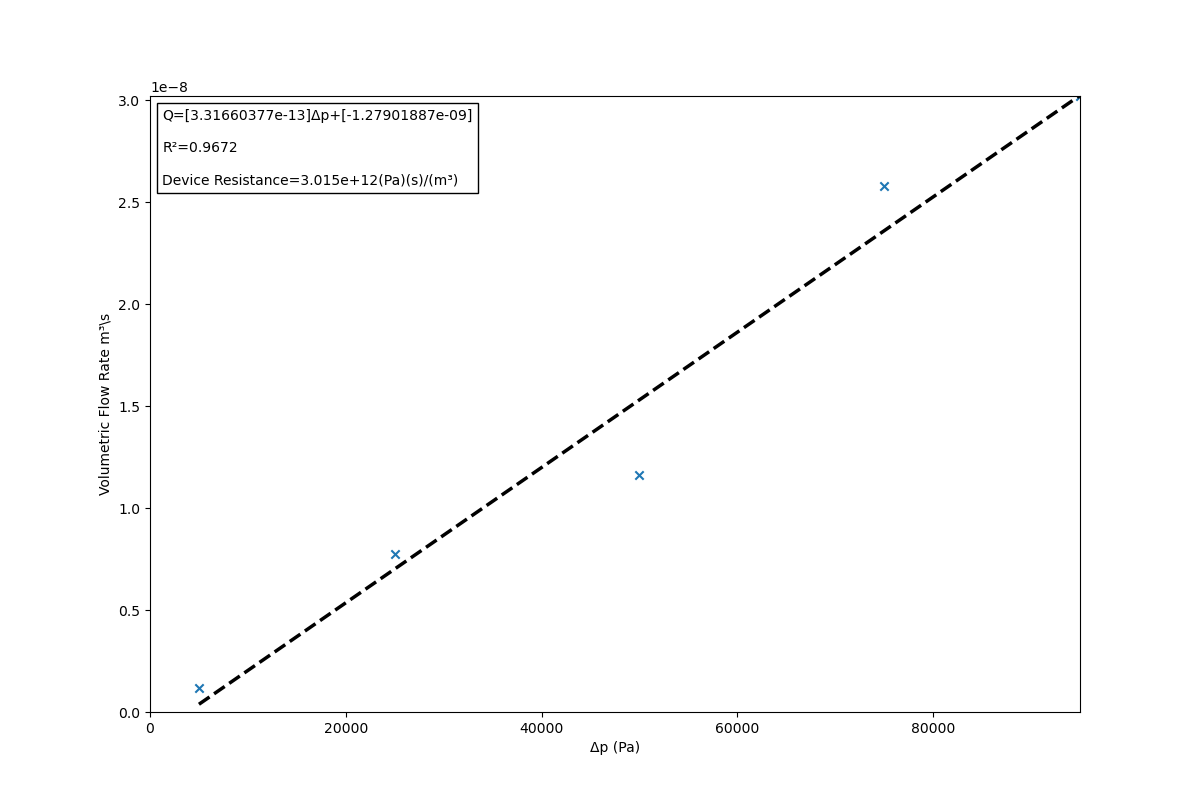
\includegraphics[width=15cm, height=10cm]{rhyd.png}
\end{center}
\noindent Hydraulic resistance is analogous to electrical resistance. As such, total hydraulic resistance in series is the sum of each `resistor'and in parallel the resistance is the sum of the reciprocal of each resistor. If we were to add a tube of a specific resistance to the above device, the total resistance would increase by the tube's hydraulic resistance $R_{tubes}$. However, the resistance of the tubes, $R_{tubes}=1\times{10^8}\left(Pa\right)\left(s\right){m^{-3}}$, is so much lower than the device's resistance it would relate to a negligible increase in resistance. \\

\noindent Given a pressure of 150mbar, we can use equation (110) to estimate Q: 

\begin{align}
    Q &= \displaystyle\frac{\Delta{p}(Pa)}{3.31660377\times{10^{13}}\nicefrac{(Pa)(s)}{m^3}} - 1.27901887\times{10^{-9}}\left(\displaystyle\nicefrac{m^3}{s}\right)\\
    Q &= \displaystyle\frac{\left(150mbar\right)\left(\displaystyle\frac{100Pa}{mbar}\right)}{3.31660377\times{10^{13}}\nicefrac{(Pa)(s)}{m^3}} - 1.27901887\times{10^{-9}}\left(\displaystyle\nicefrac{m^3}{s}\right) \\
    Q &= 3.70\times{10^{-09}}\left(\displaystyle\nicefrac{m^3}{s}\right)\hspace*{5pt}\square
\end{align}

\newpage 
\noindent We may also convert volumetric flow rate $Q=\left(\displaystyle\nicefrac{m^3}{s}\right)$ to average linear flow velocity $V_{0}=\left(\displaystyle\nicefrac{m}{s}\right)$. Doing this will allow us to calculate the Reynold's number. To perform this conversion, we must divide $Q$ by the cross-sectional area of the channel: 

\begin{align}
    V_{0} &= \displaystyle\frac{Q}{\text{\emph{channel width $\times$ channel height}}}  \\
    V_{0} &= \displaystyle\frac{3.70\times{10^{-09}}\left(\displaystyle\nicefrac{m^3}{s}\right)}{\displaystyle\frac{\left(650\mu{m}\right)\left(m\right)}{10^{6}\mu{m}}\times\displaystyle\frac{\left(30\mu{m}\right)\left(m\right)}{10^{6}\mu{m}}} \\
    V_{0} &= 0.190\left(\displaystyle\nicefrac{m}{s}\right)\hspace*{5pt}\square
\end{align}

\noindent By equation (33) the Reynolds number is: 
\begin{align*}
    Re &= \rho\left(\displaystyle\frac{L_{0}V_{0}}{\eta}\right)
\end{align*}
\noindent For non-circular channels, oftentimes hydraulic diameter $\left(D_{H}\right)$ is used in place of $L_{0}$: 

\begin{align}
    L_{0} = D_{H} = \displaystyle\frac{2{w}{h}}{w+h}
\end{align}

\noindent Substituting equations (116) \& (117) into equation (33) gives us:
\begingroup
    \addtolength\jot{5pt}
    \begin{align}
        Re &= \rho\left(\displaystyle\frac{D_{H}V_{0}}{\eta}\right) \\
        Re &= 2\times\left(\displaystyle\frac{\displaystyle\frac{\left(650\mu{m}\right)\left(m\right)}{10^{6}\mu{m}}\times\displaystyle\frac{\left(30\mu{m}\right)\left(m\right)}{10^{6}\mu{m}}}{\displaystyle\frac{\left(650\mu{m}\right)\left(m\right)}{10^{6}\mu{m}}+\displaystyle\frac{\left(30\mu{m}\right)\left(m\right)}{10^{6}\mu{m}}}\right)\times\displaystyle\frac{0.190\left(\displaystyle\nicefrac{m}{s}\right)}{\left(\displaystyle\frac{1.0(mPa)(s)\times(Pa)(s)}{10^{3}(Pa)(s)}\right)\left(\displaystyle\frac{kg}{(m)(s)}\right)}\times\left(\displaystyle\frac{998.2kg}{m^3}\right) \\
        Re &\thickapprox 10.9 \hspace*{5pt}\square
    \end{align}
\endgroup
\noindent In microfluidics, laminar flow occurs when $Re <  2000$. Therefore the experimental microfluidic device was experiencing laminar flow.

\newpage
\section{}
\begin{center}
    \large
    \textbf{Theoretical Application of an H-Filter} \\
\end{center} 
\normalsize 

\noindent The time it takes a solute with diffusion coefficient $D$ to diffuse across the width of a T-mixer is: 
\begin{align}
    T \approx \displaystyle\frac{w^2}{D}
\end{align}
\noindent And the distance travelled in that time is: 
\begin{align}
    Z = V_{0}T = \displaystyle\frac{V_{0}w^2}{D}
\end{align}
\noindent Combining equations (121) and (122) gives us the Peclet number, or the number of channel widths required for complete mixing of a solute: 
\begin{align}
    Pe = \displaystyle\frac{Z}{w}=\displaystyle\frac{V_{0}}{D}
\end{align}

\noindent In principle, T-mixers and H-filters are quite similar. However, unlike T-mixers which only have one outlet, the goal of an H-filter is to separate solutes of interest from a matrix. To understand how this works, two critical times must be taken into account: the time it takes for convective forces to induce advection of a solute compared to the time it takes for diffusive forces to induce diffusion of the solute across the width of the channel: 

\begin{align}
    \tau_{\text{conv}}&=\displaystyle\frac{L}{V_{0}} \\
    \tau_{\text{diff}}&=\displaystyle\frac{\displaystyle\left({\nicefrac{w}{2}}\right)^2}{D}=\displaystyle\frac{w^2}{4D}
\end{align}

\noindent If $\tau_{\text{conv}} \ll \tau_{\text{diff}}, \hspace*{5pt} \left(Pe<1\right)$, the solutes will largely be carried with the original buffer into the waste stream (ie advection of solute dominates). On the other hand, if $\tau_{\text{conv}} \geq  \tau_{\text{diff}}\hspace*{5pt} \left(Pe \geq 1\right)$, the solutes will be mixed into the extraction stream (ie diffusion of solute dominates). By setting $\tau_{\text{conv}}=\tau_{\text{diff}}$ and subbing equations (124) \& (125) we can derive the minimum length required for extraction of a solute: 
\begin{align}
    \tau_{\text{conv}} &= \tau_{\text{diff}} \\
    \displaystyle\frac{L}{V_{0}} &= \displaystyle\frac{w^2}{4D} \\
    L &= \displaystyle\frac{w^2{V_{0}}}{4D} \hspace*{5pt}\blacksquare
\end{align}

\noindent Given a blood sample, three fractions are of interest: dissolved ions and solutes $\left(D_{1}=2\times{10^{-9}}m^2{s^-1}\right)$, proteins $\left(D_{2}=6\times{10^{-11}}m^2{s^-1}\right)$ and red, white, and platelet cells $\left(D_{3}=2\times10^{-14}m^2{s^{-1}}\right)$. Let our theoretical H-filter have an average linear flow velocity of $V_{0}=1\left(\displaystyle\nicefrac{mm}{s}\right)$, a height of $h=20\mu{m}$ a width of $w=100\mu{m}$, and a length $\leq 50$mm. \\

\newpage
\noindent To determine the length of the H-filter needed which would only extract the dissolved ions, solutes, we would substitute $D_{1}$ into equation (128):
\begin{align}
    L &= \displaystyle\frac{\left(100\mu{m}\displaystyle\frac{m}{10^{6}\mu{m}}\right)^2\left(\displaystyle\frac{1mm}{s}\right)\left(\displaystyle\frac{m}{10^3{mm}}\right)}{4\left(2\times{10^{-9}}m^2{s^-1}\right)} \\
    L &= 1.25mm \hspace*{5pt}\square
\end{align}

\noindent If we wished to additionally extract the protein fraction, we would set $D$ to $D_{2}$, as $D_{1}\ll{D_{2}}\ll{D_{3}}$:

\begin{align}
    L &= \displaystyle\frac{\left(100\mu{m}\displaystyle\frac{m}{10^{6}\mu{m}}\right)^2\left(\displaystyle\frac{1mm}{s}\right)\left(\displaystyle\frac{m}{10^3{mm}}\right)}{4\left(6\times{10^{-11}}m^2{s^-1}\right)} \\
    L &\approx 41.7mm \hspace*{5pt}\square
\end{align}


\noindent Finally, if we wished to extract all three fractions: 
\begin{align}
    L &= \displaystyle\frac{\left(100\mu{m}\displaystyle\frac{m}{10^{6}\mu{m}}\right)^2\left(\displaystyle\frac{1mm}{s}\right)\left(\displaystyle\frac{m}{10^3{mm}}\right)}{4\left(2\times10^{-14}m^2{s^{-1}}\right)} \\
    L &= 125m \hspace*{5pt}\square
\end{align}

\noindent Given these critical lengths and the maximum length allowed, an H-filter with a length of 41.7mm would be able to extract the dissolved ions, solutes, and proteins fractions. Since diffusion is a stochastic process, 100\% recovery of the solute(s) of interest impossible. Though the H-filter can be optimized to attain near ideal extraction, the process will never recover all of the solutes. Additionally, some waste will make it through into the extraction stream and reduce the purity of the extracted solutes. 

\end{document} 